\chapter{操作系统进阶}\label{cha:latex-brief-intro}

\section{实验内容}
\begin{enumerate}
    \item 自定义一个系统调用,能够统计一个进程在执行的过程中被调度的次数。编写一个简单的用户程序,调用该自定义的系统调用,从而将进程及其调度的次数输出在屏幕上。
    \item 在实现了三个进程的优先级调度的基础上,将三个进程的循环次数从无限循环修改为有限次数,当三个进程执行完成时,计算三个进程在优先级调度算法下的周转时间、等待时间以及该系统的平均周转时间、平均等待时间和吞吐量。也可以添加新的进程,然后计算该系统的平均周转时间、平均等待时间和吞吐量。
\end{enumerate}

\section{代码分析}

\subsection{系统调用部分}
    \begin{enumerate}
        \item 系统调用过程:(以书中 write 系统调用为例),如下图 9-1 所示:
        \begin{figure}[H]
            \centering
            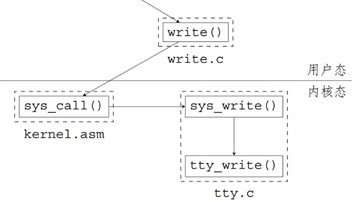
\includegraphics[width=0.8\textwidth]{figures/chapter9/9-1.jpg}
            \caption{系统调用流程图}
        \end{figure}
        
        \item 实现一个新的系统调用(这里为 get$\_$foo)主要需要完成两部分:get$\_$foo函数本身 及其内核部分 sys$\_$get$\_$foo,如图 9-2 所示:
        \begin{figure}[H]
            \centering
            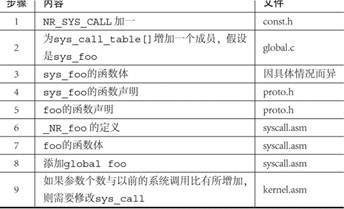
\includegraphics[width=0.8\textwidth]{figures/chapter9/9-2.jpg}
            \caption{系统调用函数}
        \end{figure}
        
        \item 添加系统调用的步骤:
        \begin{enumerate}
            \item 将 \texttt{const.h} 文件中的宏 \texttt{NR\_SYS\_CALL} 加 1。\\
            \texttt{NR\_SYS\_CALL} 表示的是操作系统中定义的系统调用的个数,会用到其值来定义系统调用数组。
            
            \item 在 \texttt{global.c} 文件为 \texttt{sys\_call\_table[]} 增加一个成员,命名为sys$\_$get$\_$foo,此处模仿前两个系统调用名并结合功能设为 \texttt{sys\_get\_num}。此处用到了步骤一中设置的 \texttt{NR\_SYS\_CALL} 来定义数组。
            
            \item 完成 \texttt{get\_foo} 的声明及 \texttt{sys\_get\_foo} 的声明和函数体。声明位于头文件 \texttt{proto.h} 中,函数体的位置较灵活,此处选择将新增的系统调用放在第一个系统调用 \texttt{sys\_get\_ticks} 后面,即 \texttt{proc.c} 文件最下方。
            
            \item 定义 \texttt{\_NR\_get\_foo} 及添加 \texttt{global get\_foo}。\\\texttt{\_NR\_get\_time equ} 后的值设为1,和已有系统调用的调用号不一致即可。
            
            \item 设计用户程序:在 \texttt{main.c} 文件中编写了测试进程:\texttt{TestA}、\texttt{TestB} 与 \texttt{TestC},如图所示。其中,\texttt{TestA} 调用了 \texttt{get\_foo} 与 \texttt{get\_ticks} 系统调用函数,进程 \texttt{B} 与进程 \texttt{C} 没有调用系统函数,目的为与 \texttt{TestA} 形成对照,使实验结果清晰,如下所示:
            \begin{lstlisting}[language = C]
    void TestA(){
        for(int k = 0;k < 10;k++){
        disp_str("A");
        disp_int(get_foo() + 1);
        disp_int(get_ticks());
        milli_delay(100);
        }
    }
            \end{lstlisting}
            \begin{lstlisting}[language = C]
    void TestB(){
        for(int i = 0;i < 10;i++){
        disp_str("B");
        milli_delay(100);
        }
    }
            \end{lstlisting}
            \begin{lstlisting}[language = C]
    void TestC(){
        for(int i = 0;i < 10;i++){
        disp_str("C");
        milli_delay(100);
        }
    }
            \end{lstlisting}
        \end{enumerate}
    \end{enumerate}


\subsection{优先级调度部分}
\begin{enumerate}
        \item 此处添加用户进程的主要步骤与系统调用部分完全一致,不重复阐述。
        
        \item 在 \texttt{main.c} 文件中给三个进程添加ticks属性,定义为有限值,每次调用ticks值减一,为0后则不再调用。并对proc.c文件中的schedule函数进行修改,删掉ticks归零后重新赋值的部分,从而将三个进程的循环次数从无限循环修改为有限次数。如下所示:
\begin{lstlisting}[language = C]
    proc_table[0].ticks = 100;
    proc_table[1].ticks = 40;
    proc_table[2].ticks = 30;
\end{lstlisting}

\begin{lstlisting}[language = C]
    /*if (!greatest_ticks){
        for (p = proc_table; p < proc_table + NR_TASKS; p++){
        p ->ticks = p-> priority;
        }
    }*/
\end{lstlisting}
        
        \item 在进程结构体中添加相应成员。周转时间命名为 \texttt{TurnaroundTick},等待时间命名为\texttt{WaitingTick}。
        此处,我对优先级调度算法进行了修改,使进程调度完全按照自行设定的优先级顺序(priority值的大小)来执行,保证高优先级进程一定在低优先级进程之前执行完毕。因此,周转时间直接读取进程结束时的ticks中,而等待时间可直接读取进程开始时的ticks。调度算法如下:
\begin{lstlisting}[language = C]
    PROCESS*	p;
    int		greatest_priority = 0;
    for (p=proc_table; p<proc_table+NR_TASKS; p++) {
		if (p->priority > greatest_priority && p->ticks > 0) {
			greatest_priority = p->priority;
			p_proc_ready = p;
		}
    }
\end{lstlisting}
        
        \item 三个进程结束后计算并打印出相应的数据,需要注意的是单位为ms,要进行转换。如下所示:
\begin{lstlisting}[language = C]
if (greatest_priority == 0) {
    // turnaround time
    disp_str("\n");
    disp_str("turnaround time of a:");
    disp_int(proc_table[0].TurnaroundTick /  10);
    disp_str("ms\n");

    disp_str("turnaround time of b:");
    disp_int(proc_table[1].TurnaroundTick /  10);
    disp_str("ms\n");

    disp_str("turnaround time of c:");
    disp_int(proc_table[2].TurnaroundTick /  10);
    disp_str("ms\n");

    // waiting time
    disp_str("waiting time of a:");
    disp_int(proc_table[0].WaitingTick /  10);
    disp_str("ms\n");

    disp_str("waiting time of b:");
    disp_int(proc_table[1].WaitingTick /  10);
    disp_str("ms\n");

    disp_str("waiting time of c:");
    disp_int(proc_table[2].WaitingTick /  10);
    disp_str("ms\n");

    // average turnaround time
    disp_str("average turnaround time:");
    disp_int((proc_table[0].TurnaroundTick + proc_table[1].TurnaroundTick + proc_table[2].TurnaroundTick / 30) / 30);
    disp_str("ms\n");
    disp_str("average waiting time:");
    disp_int((proc_table[0].WaitingTick + proc_table[1].WaitingTick + proc_table[2].WaitingTick) / 30);
    disp_str("ms\n");

    // throughput
    disp_str("throughput:");
    int timeOfThree = proc_table[0].TurnaroundTick > proc_table[1].TurnaroundTick ? proc_table[0].TurnaroundTick : proc_table[1].TurnaroundTick;
    timeOfThree = timeOfThree > proc_table[2].TurnaroundTick ? timeOfThree : proc_table[2].TurnaroundTick;
    disp_int((proc_table[0].ticks + proc_table[1].ticks + proc_table[2].ticks)/ timeOfThree);
    disp_str("/s\n");
}
\end{lstlisting}
\end{enumerate}

\section{调试过程及结果分析}
沿用之前的Makefile,以同样指令编译运行。
系统调用部分运行结果如下图9-3所示:
        \begin{figure}[H]
            \centering
            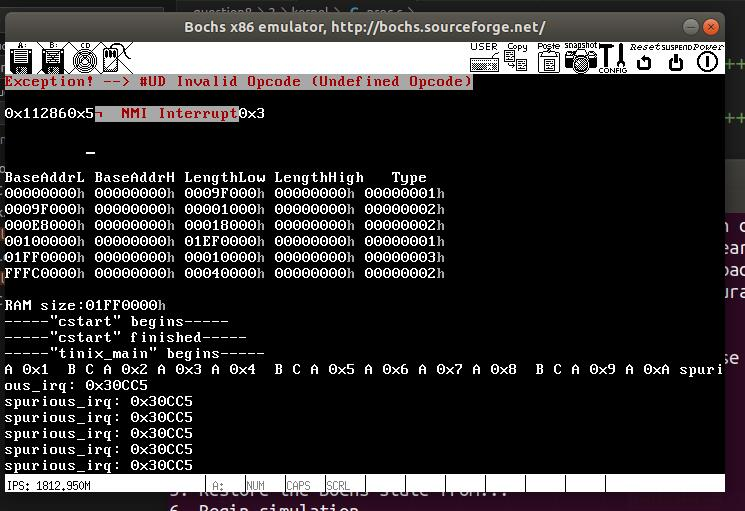
\includegraphics[width=0.8\textwidth]{figures/chapter9/9-3.jpg}
            \caption{系统调用运行结果}
        \end{figure}
优先级调度部分运行结果如下图9-4所示:
        \begin{figure}[H]
            \centering
            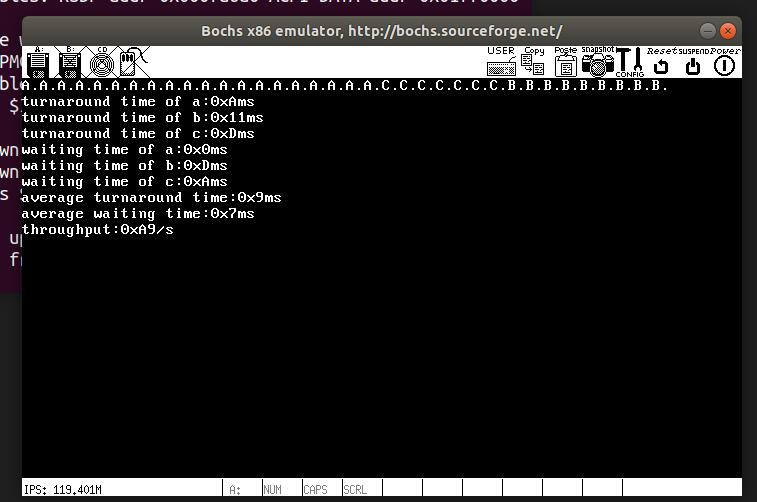
\includegraphics[width=0.8\textwidth]{figures/chapter9/9-4.jpg}
            \caption{优先级调度运行结果}
        \end{figure}
\section{实验总结}
最后的操作系统进阶实验中,首先在内核中添加了一个新的系统调用,该系统调用功能是统计一个进程在执行过程中被调度的次数,然后在用户程序中调用该系统调用。在实现了自定义的系统调用的基础上,我设计了一个简单的进程优先级调度算法。原先的三个进程是无限循环执行的,我将它们的循环次数修改为有限次数。三个进程执行完成后,我计算了它们在优先级调度算法下的周转时间、等待时间以及整个系统的平均周转时间、平均等待时间和吞吐量。通过这次实验,我学会了如何在操作系统中添加自定义的系统调用,熟悉了整个系统调用的流程,并且了解了系统调用的原理和使用方法,同时更深入地理解了进程调度算法的原理和实际应用。\par


